\section{Modules}
\label{sec:modules}

This section provides an overview of the main modules that are used in
an SRAM.  For each module, we will provide both an architectural
description and an explanation of how that design is generated and
used in OpenRAM.  The modules described below are provided in the
first release of OpenRAM, but by no means is this an exhaustive list
of the possible circuits that can be adapted into a SRAM architecture;
refer to Section~\ref{sec:implementation} for more information on
adding different module designs to the compiler.

Data structures for schematic and layout are provided in the
\verb|base| directory. These implement a generic design object and
have many auxiliary functions for routing, pin access, placement,
DRC/LVS, etc.  These are discussed further in
Section~\ref{sec:implementation}.

Each module has a corresponding Python class in the
\verb|compiler/modules| directory.  These classes are used to generate
both the GDSII layout and spice netlists. A module can consist of
hard library cells (Section~\ref{sec:techdir}), paramterized
cells (Section~\ref{sec:parameterized}) or other modules.

When combining modules at any level of hierarchy, DRC rules for
minimum spacing of metals, wells, etc. must be followed and DRC and
LVS are run by default after each hierarchical module's creation. A
module is responsible for creating its own pins to enable routing
at the next level up in the hierarchy. A module must also define its
height and width assuming a (0,0) offset for the lower-left coordinate
to aid with placement.


\subsection{The Bitcell and Bitcell Array}
\label{sec:bitcellarray}

OpenRAM can work with any cell as the bitcell. This could be a foundry
created one or a user design rule cell for experiments.  In addition,
it could be a common 6T cell or it could be replaced with an 8T, 10T
or other cell, depending on needs.

By default, OpenRAM uses a standard 6T cell as shown in 
Figure~\ref{fig:6t_cell}.  The cross coupled inverters hold a single
data bit that can either be driven into, or read from the cell by the
bitlines.  The access transistors are used to isolate the cell from
the bitlines so that data is not corrupted while a cell is not being
accessed.

\begin{figure}[h!]
\centering
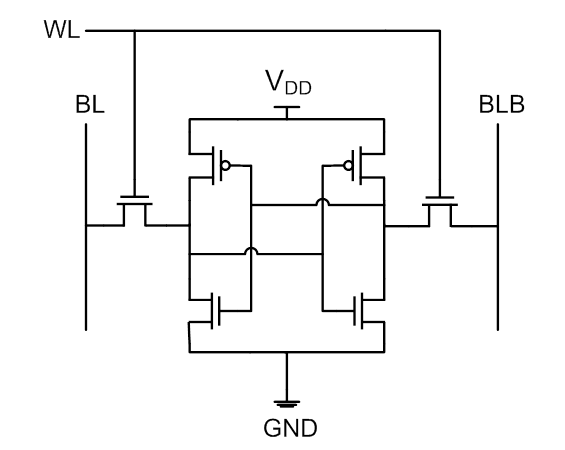
\includegraphics[scale=.9]{figs/cell_6t_schem.pdf}
\caption{Standard 6T cell.}
\label{fig:6t_cell}
\end{figure}

% tiling memory cells
The 6T cells are tiled together in both the horizontal and vertical
directions to make up the memory array.  

% keeping it square
It is common practice to keep the aspect ratio of a memory array
roughly ``square'' to ensure that the bitlines and wordlines do not
become too long. If the bitlines are too long, this can increase the
bitline capacitance, slow down the operation and lead to bitline
leakage problems.  To make an array ``more square'', multiple words
can share rows by interleaving the bits of each word. The column mux
in Section~\ref{sec:column_mux} is responsbile for selecting a subset
of bitcells in a row to extract a word during read and write
operations.

% memory cell is a library cell
In OpenRAM, we provide a library cell for the 6T cell that can be
swapped with a fab memory cell, if available. The transitors in the
cell are sized appropriately considering read and write noise margins.

% bitcell and bitcell_array classes
The bitcell class in \verb|modules/bitcell.py| is a single
memory cell and is usually a pre-made library cell.

% bitcell_array
The bitcell\_array class in \verb|modules/bitcell_array.py| dynamically
implements the memory cell array by instantiating a the bitcell class
in rows and columns.

% abutment connections
During the tiling process, bitcells are abutted so that all bitlines
and word lines are connected in the vertical and horizontal directions
respectively. This is done by using the boundary layer to define the
height and width of the cell. If this is not specified, OpenRAM will
use the bounding box of all shapes as the boundary. The boundary layer
should be offset at (0,0) in the lower left coordinate.

% flipping
In order to share supply rails, bitcells are flipped in alternating
rows. 



\subsection{Precharge Circuitry}
\label{sec:precharge}

The precharge circuit is depicted in Figure~\ref{fig:precharge} and is
implemented by three PMOS transistors. The input signal to the cell,
clk, enables all three transistors during the first half of a read or
write cycle (i.e. while the clock signal is low).  M1 and M2 charge bl
and br to vdd while M3 equalizes the voltages seen between the bitlines.

\begin{figure}[h!]
\centering
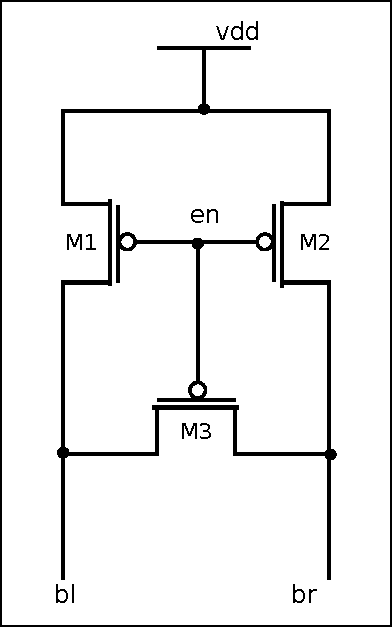
\includegraphics[width=5cm]{./figs/precharge_schem.pdf}
\caption{Schematic of a precharge circuit.}
\label{fig:precharge}
\end{figure}

In OpenRAM, the precharge citcuitry is dynamically generated using the
parameterized transistor class ptx which is further discussed in
Section~\ref{sec:ptx}. The offsets of the bitlines and the width of
the precharge cell are equal to the bitcell so that the bitlines are
correctly connected by abutment. The precharge class in
\verb|modules/precharge.py| dynamically generates a single precharge
cell.

\verb|modules/precharge_array.py| creates a row of precharge cells at
the top of a bitcell array.




\subsection{Address Decoders}
\label{sec:address_decoder}

The address decoder deodes the binary-encoded row address bits from the
address bus as inputs, and asserts a one-hot wordline in the row that
data is to be read or written. OpenRAM provides a hierarchical address
decoder as the default, but will soon have other options.

The address decoders are created using parameterized gates (pnand2,
pnand3, pinv) and transistors (ptx). This means that the decoders do
not rely on any hard library cells.

\subsubsection{Hierarchical Decoder}
\label{sec:hierdecoder}


A simple 2:4 decoder is shown in Figure~\ref{fig:2:4decoder}. This
decoder computes all of the possible decode values using a single
level of nand gates along with the inverted and non-inverted inputs.
As the decoder size increases the size of the nand gates required for
decoding would increase proportional to the bits to be decoded.  This
would not be practical for large decoders.


\begin{figure}[h!]
\centering
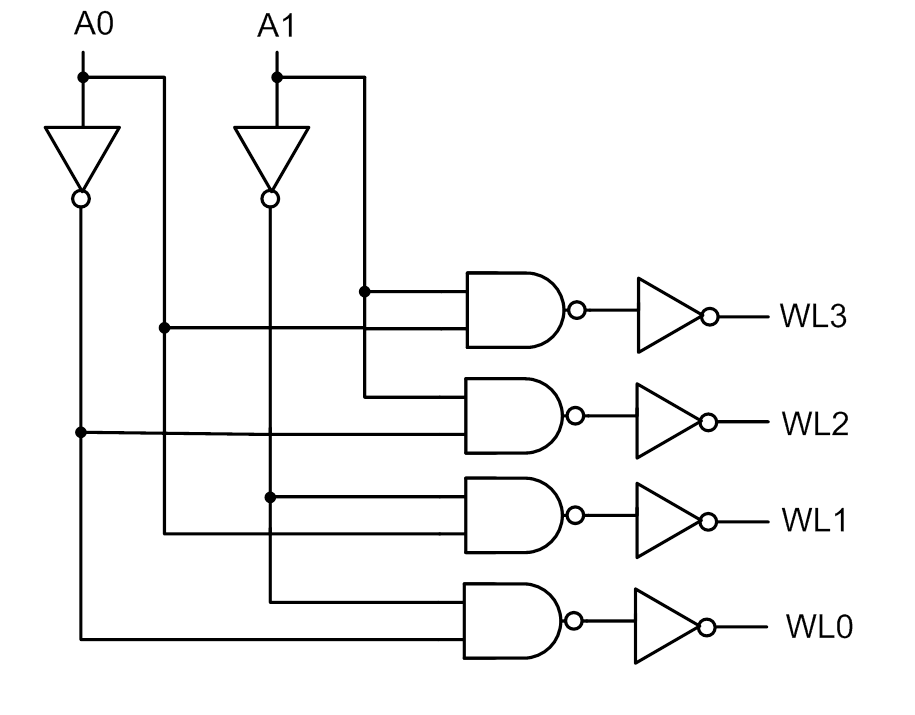
\includegraphics[scale=.6]{./figs/2t4decoder.pdf}
\caption{Schematic of 2-4 simple decoder.}
\label{fig:2:4decoder}
\end{figure}

A hierarchical decoder uses two-levels of decoding hierarchy to
perform an address decode. The first stage computes predecoded values
while the second stage computes the final decoded values.
Figure~\ref{fig:4 to 16 decoder} shows a 4:16 heirarchical
decoder. The decoder uses two 2:4 decoders for
predecoding and 2-input nand gates and inverters for final decoding to
form the 4:16 decoder.

\begin{figure}[h!]
\centering
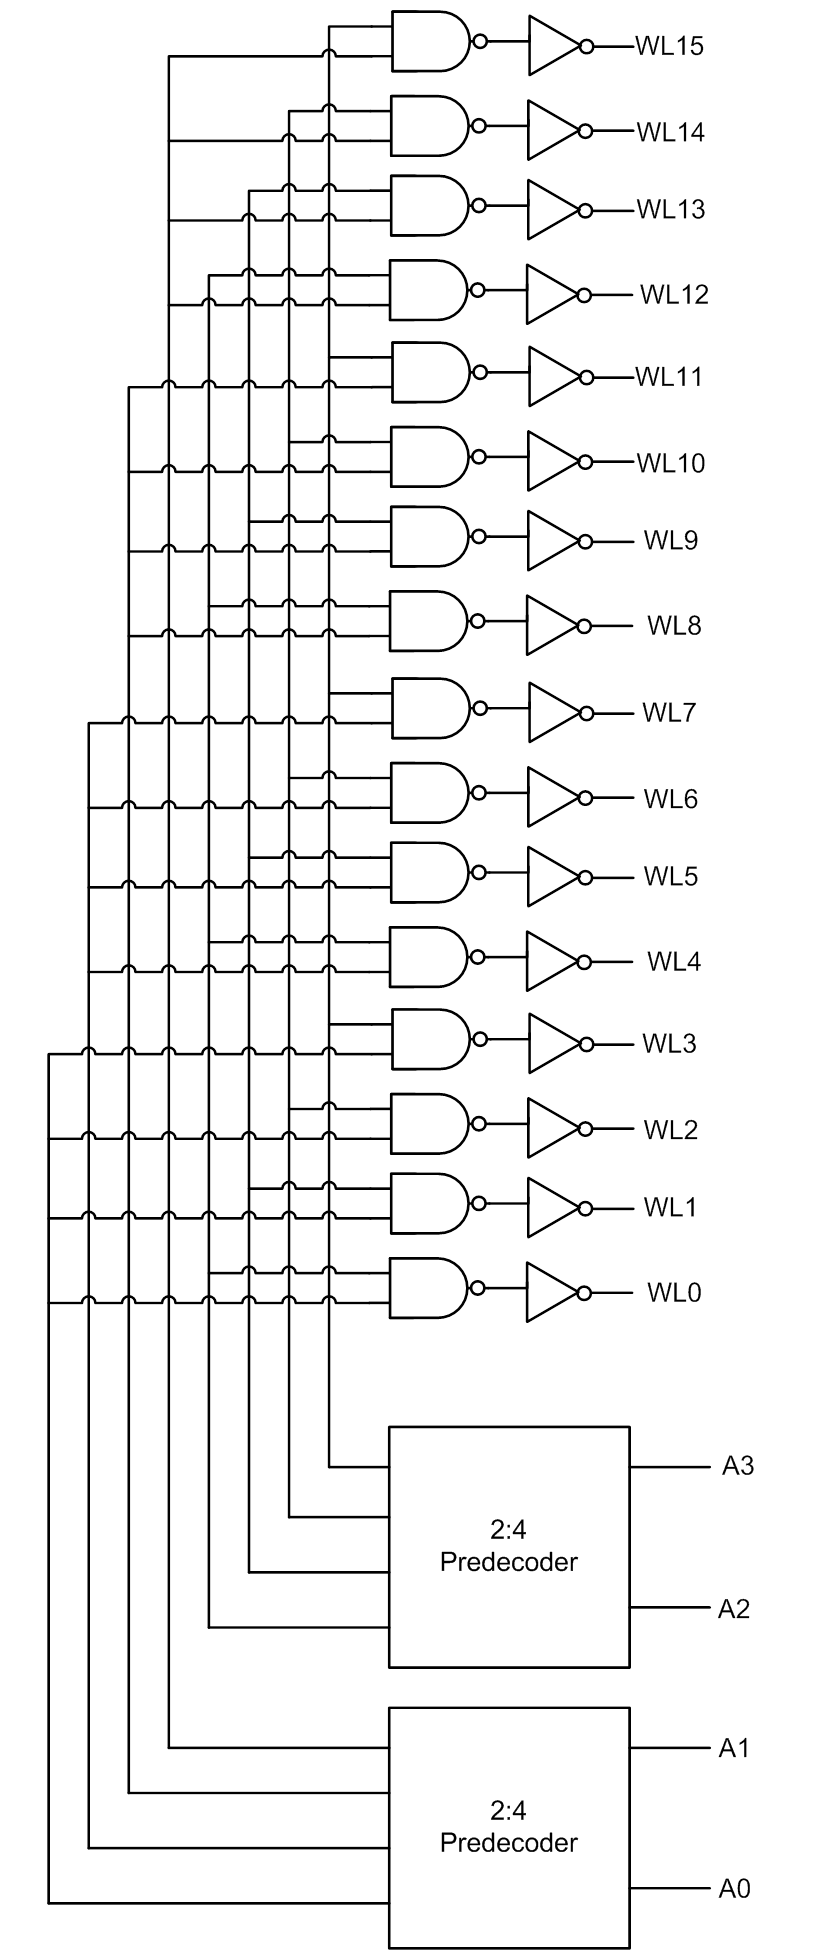
\includegraphics[scale=.6]{./figs/4t16decoder.pdf}
\caption{Schematic of 4:16 hierarchical decoder.}
\label{fig:4 to 16 decoder}
\end{figure}

The predecoder generates a total of 8 intermediate signals from the
address bits and their complements. These intermediate signals are in
two groups of 4 from each decoder. The enumeration of all 4 x 4
predecoded values are used by the final decode to produce the 16
decoded results.  As an example, Table~\ref{table:4-16 hierarchical_decoder}
gives the detailed input and output siganls for the 4:16 hierarchical
decoder.


 \begin{table}[h!] 
   \begin{center}
     \begin{tabular}{| c | c | c | c |}
     \hline
     A[3:0] & predecoder1 & predecoder2 & Selected WL\\ \hline
     0000 & 1000 & 1000 & 0\\ \hline
     0001 & 1000 & 0100 & 1\\ \hline
     0010 & 1000 & 0010 & 2\\ \hline
     0011 & 1000 & 0001 & 3\\ \hline
     0100 & 0100 & 1000 & 4\\ \hline
     0101 & 0100 & 0100 & 5\\ \hline
     0110 & 0100 & 0010 & 6\\ \hline
     0111 & 0100 & 0001 & 7\\ \hline
     1000 & 0010 & 1000 & 8\\ \hline
     1001 & 0010 & 0100 & 9\\ \hline
     1010 & 0010 & 0010 & 10\\ \hline
     1011 & 0010 & 0001 & 11\\ \hline
     1100 & 0001 & 1000 & 12\\ \hline
     1101 & 0001 & 0100 & 13\\ \hline
     1110 & 0001 & 0010 & 14\\ \hline
     1111 & 0001 & 0001 & 15\\ \hline
     \end{tabular}
   \end{center}
   \caption{Truth table for 4:16 hierarchical decoder.}
   \label{table:4-16 hierarchical_decoder}
 \end{table}


As the address size increases, additional sizes of pre- and final
decoders can be used.  In OpenRAM, there are implementations for
\verb|modules/hierarchical\_predecode2x4.py| and
\verb|modules/hierarchical\_predecode3x8.py| to produce 2:4 and 3:8
predecodes, respectively. These same decoders are used to generate the
column mux select bits as well.

For the final decode, we can use either pnand2 or pnand3 gates. This
allows a maximum size of three 3:8 predocers along with a final pnand3 decode
stage, or, 512 word lines. To extend beyond this, a pnand4 or
a 4:16 predecoder would be needed.


\subsection{Wordline Driver}
\label{sec:wldriver}

The word line driver buffers the address decoder to drive the wordline and
gates the signal until the decode has stabilized. Without waiting, an
incorrectly asserted wordline could erase memory contents.
The word line driver is sized according to the bitcell array width so
that wordlines in larger memory arrays can be appropriately driven.

% gating for first half decode, second half read/write
The first half of the clock cycle is used for address decoding in
OpenRAM.  Therefore, the wordline driver is enabled in the second half
of the clock cycle in OpenRAM.  The buffered clock signal drives each
wordline driver row and is logically ANDed with the decoder output.

% bank clock gating for wordline driver
In multi-bank structures the clock buffer is also anded with the bank
select signal to prevent the read/writing of an entire bank.

\begin{figure}[h!]
\centering
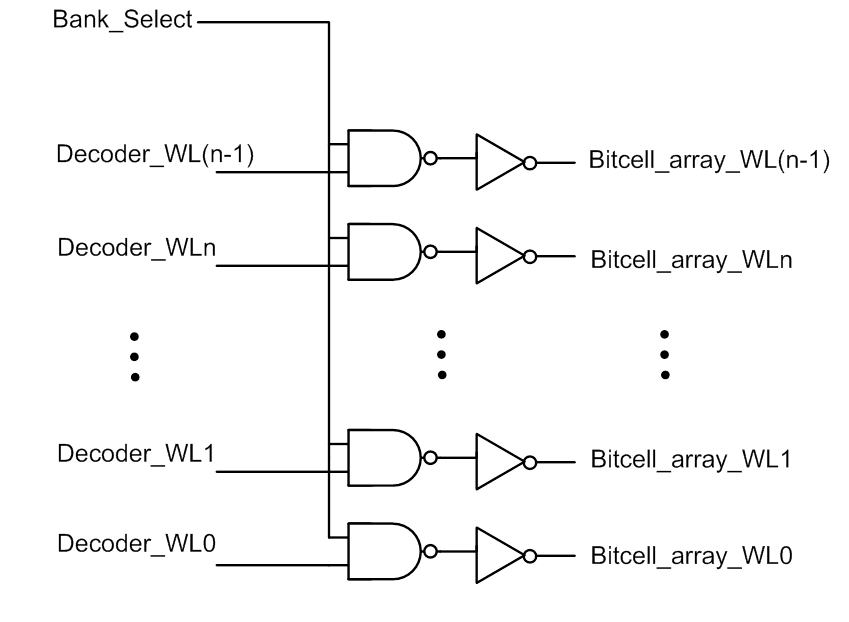
\includegraphics[scale=.6]{./figs/wordline_driver.pdf}
\caption{Diagram of word line driver.}
\label{fig:wordline_driver}
\end{figure}

Figure~\ref{fig:wordline_driver} illustrates the wordline driver and
its inputs/outputs. This is implemented in the
\verb|modules/wordline_driver.py| module and matches the number of
rows in the bitcell array of a bank.

OpenRAM creates the wordline drivers using the parameterized pinv and
pnand2 classes. This enables the wordline driver to be matched to the
bitcell height and to sized to drive the wordline load.



\subsection{Column Mux}
\label{sec:column_mux}
The column mux is an optional module in an SRAM bank. Without a column
mux, the bank is assumed to have a single word in each row. A column
mux enables more more than one word to be stored in each row and
read/written individually.  The column mux is used for both the read
and write operations by connecting the bitlines of a bank to
both the sense amplifier and the write driver.

In OpenRAM, the column mux uses the {\bf high address bits} to select
the appropriate word in each row.  If n-bits are used, there are $2^n$
words in each row. OpenRAM currently allows 2, 4, or 8 words per row,
but the 8 words are not fully debugged (as of 2/12/18).

%% OpenRAM provides several options for column mux, but the default
%% is a single-level column mux which is sized for optimal speed.

%% \subsubsection{Tree\_Decoding Column Mux}
%% \label{sec:tree_decoding_column_mux}

%% The schematic for a 4-1 tree
%% multiplexer is shown in Figure~\ref{fig:colmux}.

%% \begin{figure}[h!]
%% \centering
%% 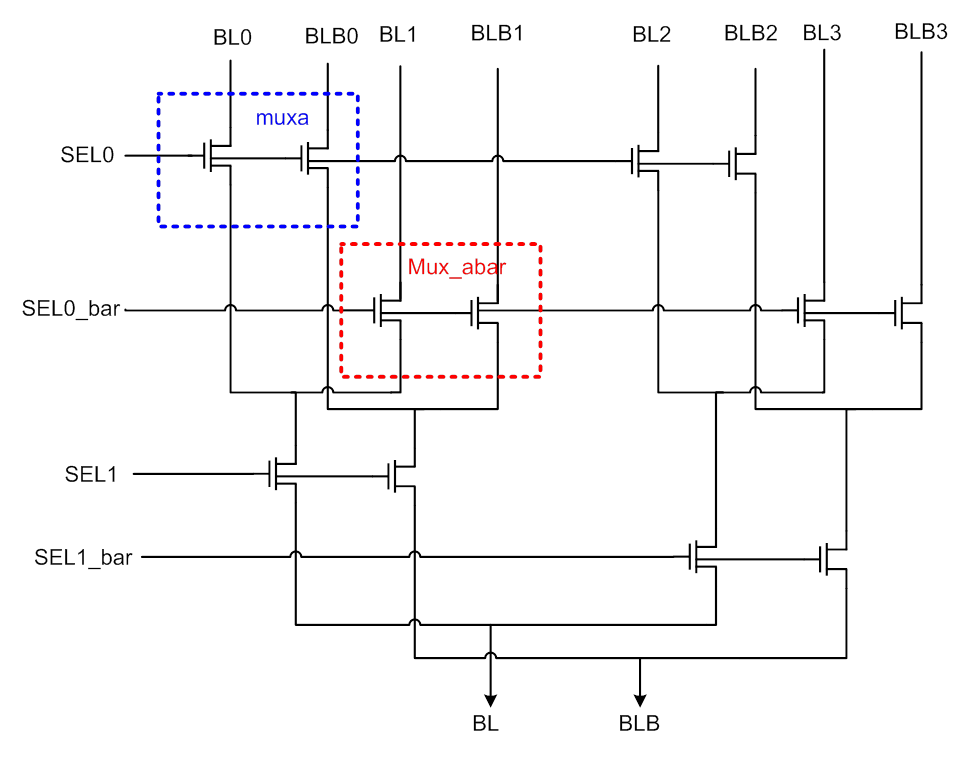
\includegraphics[scale=.9]{./figs/tree_column_mux_schem.pdf}
%% \caption{Schematic of 4-1 tree column mux that passes both of the bitlines.}
%% \label{fig:colmux}
%% \end{figure}

%% \fixme{Shading/opacity is different on different platforms. Make this a box in the image. It doesn't work on OSX.}

%% This tree mux selects pairs of bitlines (both BL and BL\_B) as inputs
%% and outputs.  This 4-1 tree mux illustrates the process of choosing
%% the correct bitlines if there are 4 words per row in the memory array.
%% Each bitline pair represents a single bit from each word.  A binary
%% reduction pattern, shown in Table~\ref{table:colmux}, is used to
%% select the appropriate bitlines.  As the number of words per row in
%% the memory array increases, the depth of the column mux grows.  The
%% depth of the column mux is equal to the number of bits in the column
%% address bus.  The 4-1 tree mux has a depth of 2.  In level 1, the
%% least significant bit from the column address bus selects either the
%% first and second words or the third and fourth words.  In level 2, the
%% most signifant column address bit selects one of the words passed down
%% from the previous level.  Relative to other column mux designs, the
%% tree mus uses significantly less devices.  But, this type of design
%% can provide poor performance if a large decoder with many levels are
%% needed.  The delay of of a tree mux quadratically increases with each
%% level.  Due to this fact, other types of column
%% decoders should be considered for larger arrays.

%% \begin{table}[h!] 
%%   \begin{center}
%%     \begin{tabular}{| c | c | c | c |}
%%     \hline
%%     Selected BL & Inp1 & Inp2 & Binary\\ \hline
%%     BL0 & SEL0\_bar & SEL1\_bar & 00\\ \hline
%%     BL1 & SEL0 & SEL1\_bar & 01\\ \hline
%%     BL2 & SEL0\_bar & SEL1 & 10\\ \hline
%%     BL3 & SEL0 & SEL1 & 11\\
%%     \hline
%%     \end{tabular}
%%   \end{center}
%%   \caption{Binary reduction pattern for 4-1 tree column mux.}
%%   \label{table:colmux}
%% \end{table} 

%% In OpenRAM, the tree column mux is a dynamically generated design.  The
%% \verb|tree_mux_array| is made up of two dynamically generated cells: \verb|muxa|
%% and \verb|mux_abar|.  The only diffference between these cells is that input
%% select signal is either hooked up to the \textbf{SEL} or
%% \textbf{SEL\_bar} signals (see highlighted boxes in
%% Figure~\ref{fig:colmux}).  These cells are initialized the the
%% \verb|column_muxa| and \verb|column_muxabar| classes in \verb|columm_mux.py|.  Instances
%% of \verb|ptx| PMOS transistors are added to the design and the necessary
%% routing is performed using the \verb|add_rect()| function. A horizontal rail
%% is added in metal2 for both the SEL and Sel\_bar signals.  Underneath
%% those input rails, horizontal straps are added.  These straps are used
%% to connect the BL and BL\_B outputs from \verb|muxa| to the BL and BL\_B
%% outputs of \verb|mux_abar|.  Vertical conenctors in metal3 are added at the
%% bottom of the cell so that connections can be made down to the sense
%% amp.  Vertical connectors are also added in metal1 so that the cells
%% can connect down to other mux cells when the depth of the tree mux is
%% more than one level.

%% The \verb|tree_mux_array| class is used to generate the tree mux.
%% Instances of both the \verb|muxa| and \verb|mux_abar| cells are instantiated and
%% are tiled row by row.  The offset of the cell in a row is determined
%% by the depth of that row in the tree mux.  The pattern used to
%% determine the offset of the mux cells is
%% $muxa.width*(i)*(2*row\_depth)$ where is the column number.  As the
%% depth increases, the mux cells become further apart.  A separate
%% ``for'' loop is invoked if the $depth>1$, which extends the
%% power/ground and select rails across the entire width of the array.
%% Similarly, if the $depth>1$, spice net names are created for the
%% intermediate connection made at the various levels.  This is necessary
%% to ensure that a correct spice netlist is generated and that the
%% input/output pins of the column mux match the pins in the modules that
%% it is connected to.


\subsubsection{Single-Level Column Mux}
\label{sec:single_level_column_mux}

OpenRAM includes a single-level pass-gate mux implemtation for the
column mux.  A single level of NMOS devices is driven by either the
input address (and it's complement) or decoded input addresses using a
2:4 predecoder (Section~\ref{sec:hierdecoder}).

Figure~\ref{fig:2t1_single_level_column_mux} shows the schematic of a
2:1 single-level column mux. In this column mux, the {\bf MSB of the
  address bus} and it's complement drive the pass transistors.

Figure~\ref{fig:4t1_single_level_column_mux} shows the schematic of a
4:1 single-level column mux. The select bits are decoded from the {\bf
  2 MSB of the address bus} using a 2:4 decoder.  The 2:4 decoder
provides one-hot select signals to select one column.

In OpenRAM, one mux, single\_level\_mux, is dynamically generated in
\verb|modules/single_level_column_mux.py| and multiple of these muxes
are tiled together in \verb|modules/single_level_column_mux_array.py|.

single\_level\_mux uses the parameterized ptx (Section~\ref{sec:ptx}
to generate 2 or 4 NMOS transistors for each the bl and br
bitlines. Horizontal rails are added for the $sel$ signals.  The
bitlines are automatically pitch-matched to the bitcell array.


\begin{figure}[h!]
\centering
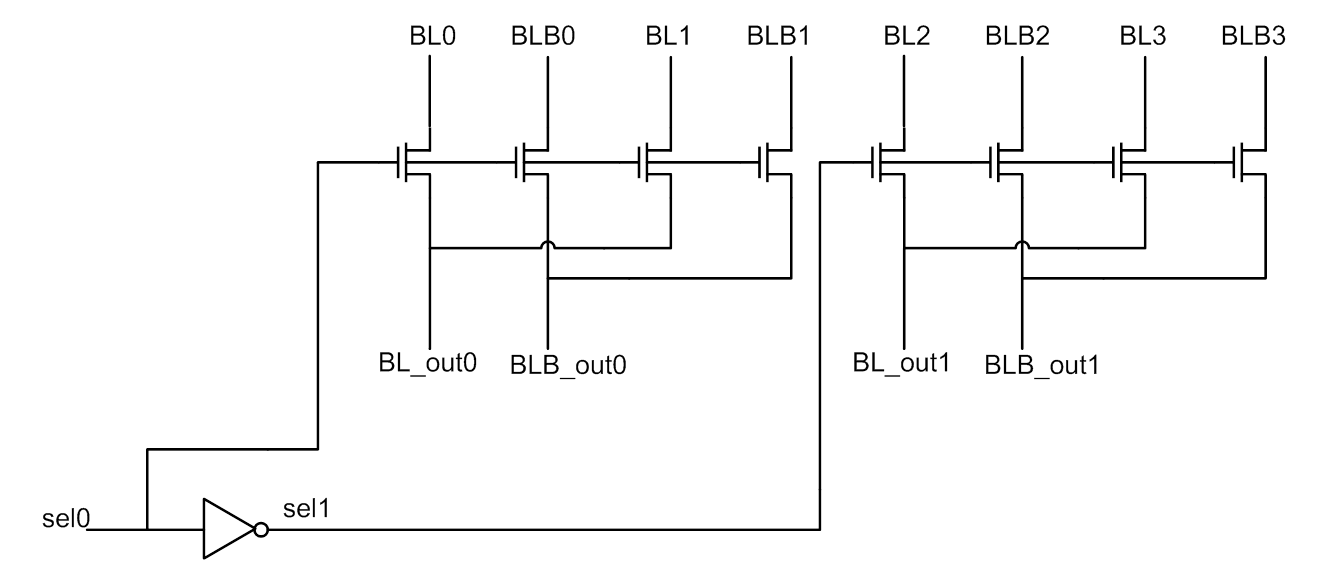
\includegraphics[scale=.5]{./figs/2t1_single_level_column_mux.pdf}
\caption{Schematic of a 2:1 single level column mux. \fixme{Signals names are wrong.}}
\label{fig:2t1_single_level_column_mux}
\end{figure}



\begin{figure}[h!]
\centering
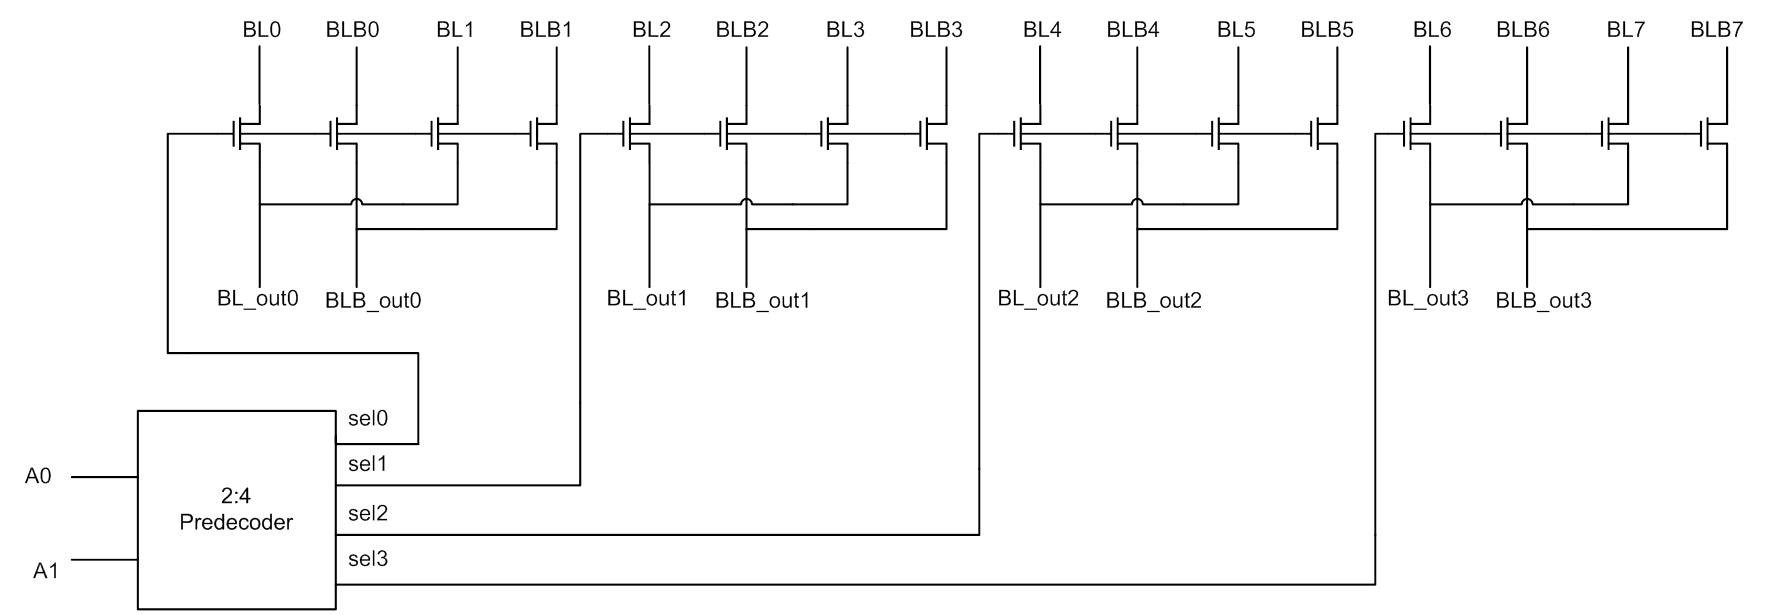
\includegraphics[scale=.5]{./figs/4t1_single_level_column_mux.pdf}
\caption{Schematic of a 4:1 single level column mux. \fixme{Signals names are wrong.}}
\label{fig:4t1_single_level_column_mux}
\end{figure}


\subsection{Sense Amplifier}
\label{sec:senseamp}
The sense amplifier is used to sense the difference between the
bitline and bitline bar while a read operation is performed.
The sense amplifier also includes two PMOS transistors for bitline
isolation to speed-up read operations. The schematic for the sense amp is shown in
Figure~\ref{fig:sense_amp}.

\begin{figure}[h!]
\centering
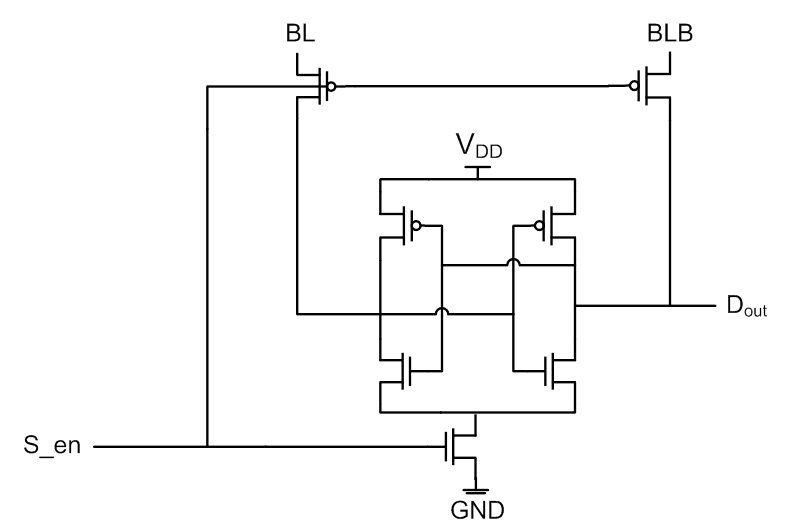
\includegraphics[scale=.8]{./figs/sense_amp_schem.pdf}
\caption{Schematic of a single sense amplifier cell.}
\label{fig:sense_amp}
\end{figure}

During address decoding (while the wordline is not asserted), the sense
amplifier is disabled and the bitlines are precharged to vdd by the
precharge unit. The two PMOS transistors also connect the bitlines to the sense amplifier.

The en signal comes from the control logic (Section~\ref{sec:control})
including the timing and replica bitline (Section~\ref{sec:RBL}). It
is only enabled after sufficient swing is seen on the bitlines so that
the value can be accurately sensed.

The sense amplifier is enabled by the en signal, which initiates the
read operation, and also isolates the sense amplifier from the
bitlines.  This allows the sense amplifier to drive a smaller
capacitance rather than the whole bitline.  At this time, the footer
transistor is also enabled which allows the sense amplifier to use
feedback to sense the bitline differential voltage.

When the sense amp is enabled, one of the bitlines experiences a
voltage drop based on the value stored in the memory cell.  If a zero
is stored, the bitline voltage drops.  If a one is stored, the bitline
bar voltage drops.  The output signal is then
taken to a true logic level and latched for output to the data bus.

In OpenRAM, the sense amplifier is a libray cell.  The associated
layout and spice netlist can be found in the \verb|gds_lib| and
\verb|sp_lib| in the technology directory. The sense\_amp class in
\verb|modules/sense_amp.py| is a single instance of the sense amp
library cell.


The sense\_amp\_array class in \verb|modules/sense_amp_array.py|
handles the tiling of the sense amps cells.  One sense amp cell is
needed per data bit and the sense amp cells need to be appropriately
spaced so that they can hook up to the column mux bitline pairs.  The
spacing is determined based on the number of words per row in the
memory array.  

The sense amp is a library cell so that custom
amplifier designs could be swapped into the memory as needed.  The two
major things that need to be considered while designing the sense
amplifier cell are the size of the cell and the bitline/input pitches.
Optimally, the cell should be no wider than the 6T cell so that it
abuts to the column mux and no extra routing or space is needed.
Also, the bitline inputs of the sense amp need to line up with the
outputs of the write driver.  In the current version of OpenRAM, the
write driver is situated under the sense amp, which had bitlines
spaning the entire height of the cell.  In this case, the sense
amplifier is disabled during a write operation but the bitlines still
connect the write driver to the column mux without any extra routing.


\subsection{Write Driver}
\label{sec:writedriver}

The write driver is used to drive the input signal into the memory
cell during a write operation.  It can be seen in
Figure~\ref{fig:write_driver} that the write driver consists of two
tristate buffers, one inverting and one non-inverting.  It takes in a
data bit, from the data bus, and outputs that value on the bitline,
and its complement on bitline bar.  The bitlines need to be
complements so that the data value can be correctly stored in the 6T
cell. Both tristates are enabled by the EN signal.

\begin{figure}[h!]
\centering
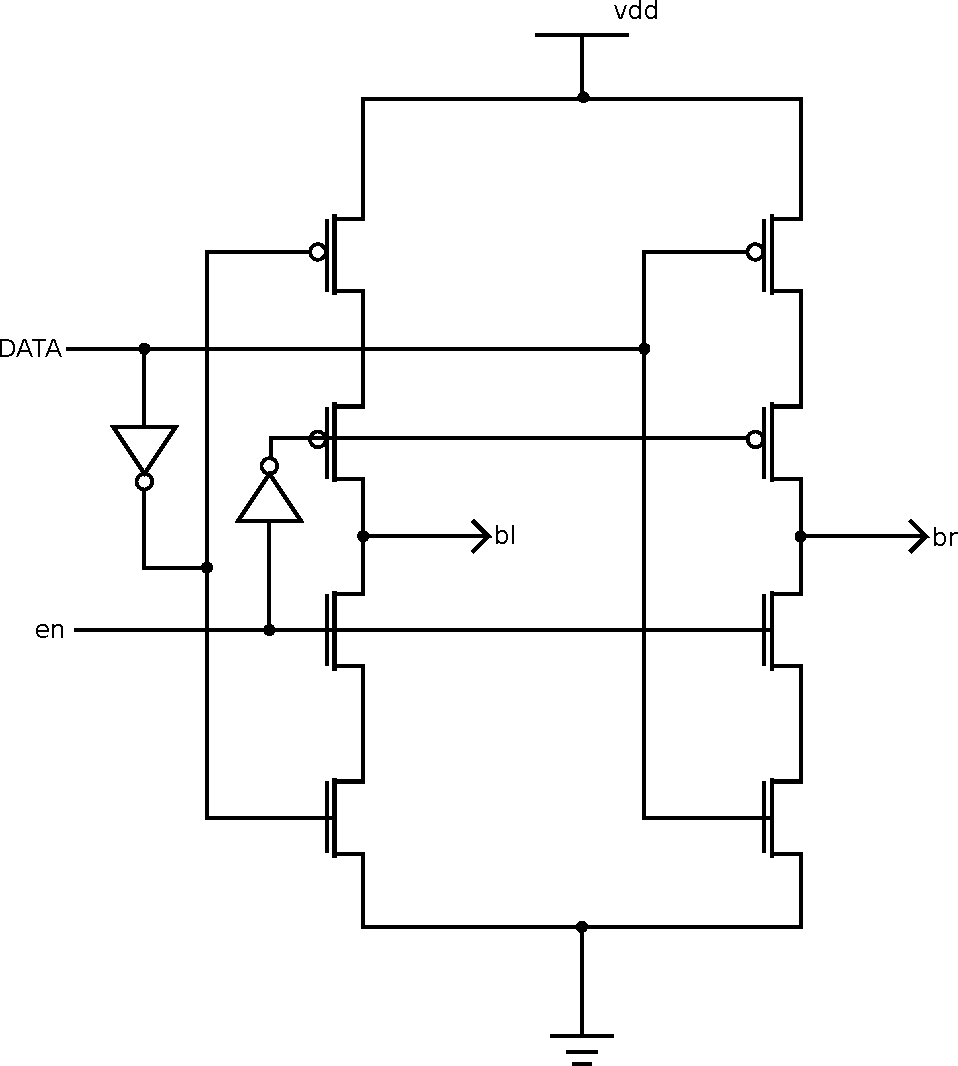
\includegraphics[scale=.8]{./figs/write_driver_schem.pdf}
\caption{Schematic of a write driver cell, which consists of 2 tristates (non-inverting and inverting) to drive the bitlines.}
\label{fig:write_driver}
\end{figure}

Currently, in OpenRAM, the write driver is a library cell.  The
associated layout and spice netlist can be found in the \verb|gds_lib| and
\verb|sp_lib| in the FreePDK45 directory.  Similar to the \verb|sense_amp_array|,
the \verb|write_driver_array| class tiles the write driver cells.  One
driver cell is needed per data bit and Vdd, Gnd, and EN signals must
be extended to span the entire width of the cell. It is not optimal to
have the write driver as a library cell because the driver needs to be
sized based on the capacitance of the bitlines.  A large memory array
needs a stronger driver to drive the data values into the memory
cells.  We are working on creating a parameterized tristate class,
which will dynamically generate write driver cells of different
sizes/strengths.

\subsection{Flip-Flop Array}

In a synchronous SRAM it is necessary to synchronize the inputs and
outputs with a clock signal by using flip-flops.  In FreePDK45 we
provide a library cell for a simple master-slave flip-flop, see
schematic in Figure~\ref{fig:ms_flop}.  In our library cell we provide
both Q and Q\_bar as outputs of the flop because inverted signals are
used in various modules.  The \verb|ms_flop| class in \verb|ms_flop.py|
instatitates a single master-slave flop, and the \verb|ms_flop_array| class
generates an array of flip-flops.  Arrays of flops are necessary for
the data bus (an array for both the inputs and outputs) as well as the
address bus (an array for row and column inputs).  The \verb|ms_flop_array|
takes the number of flops and the type of array as inputs.  Currently,
the type of the array must be either ``data\_in'', ``data\_out'',
``addr\_row'', or ``addr\_col'' verbatim.  The array type input is
used to look up that associated pin names for each of the flop arrays.
This was implemented very quickly and should be improved in the near
future...

\begin{figure}[h!]
\centering
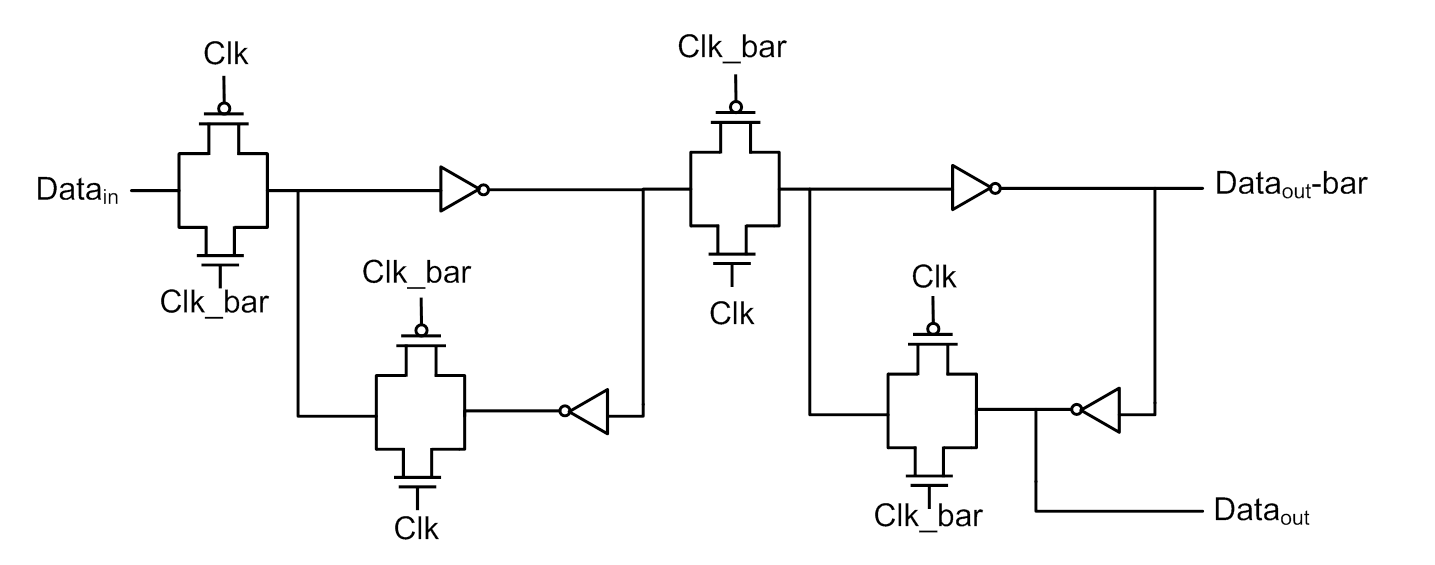
\includegraphics[scale=.7]{./figs/ms_flop_schem.pdf}
\caption{Schematic of a master-slave flip-flop provided in FreePDK45 library}
\label{fig:ms_flop}
\end{figure}

\subsection{Control Logic}

The details of the control logic architecture are outlined in
Section~\ref{sec:control}.  The control logic module,
\verb|control_logic.py|, instantiates a \verb|control_logic| class that arranges
all of the flip-flops and logic associated with the control signals
into a single module. Flip-flops are instantiated for each control
signal input and library NAND and NOR gates are used for the logic.  A
delay chain, of variable length, is also generted using parameterized
inverters.  The associated layouts and spice netlists can be found in
the \verb|gds_lib| and \verb|sp_lib| in the FreePDK45 directory.

\section{Bank and SRAM}
\label{sec:bank}

The overall memory architecture is shown in figure~\ref{fig:bank}.
As shown in this figure one Bank contains different modules including 
precharge-array which is positioned above the bitcell-array, 
column-mux-array which is located below the bitcell-array, 
sense-amp-array, write-driver-array, data-in-ms-flop-array 
to synchronize the input data with negative edge of the clock, 
tri-gata-array to share the bidirectional data-bus between input 
and output data, hierarchical decoder which is placed on the right side 
of the bitcell-array (predecoder + decoder), wordline-driver which drives 
the wordlines horizontally across the bitcell-array and address-ms-flops 
to synchronize the input address with positive edge of the clock. 

In bitcell-array each memory cell is mirrored vertically and horizontally inorder to share VDD and GND rails with adjacent cells and form the array. 
Data-bus is connected to tri-gate, address-bus is connected to address-ms-flops and bank-select 
signal will enable the bank when it goes high. To complete the SRAM design, bank is connected to control-logic as shown in figure~\ref{fig:bank}. 
Control-logic controls the timing 
of modules inside the bank. CSb, OEb, Web and clk are inputs to the control logic and output of 
control logic will ANDed with bank-select signal and send to the corresponding modules.


\begin{figure}[h!]
\centering
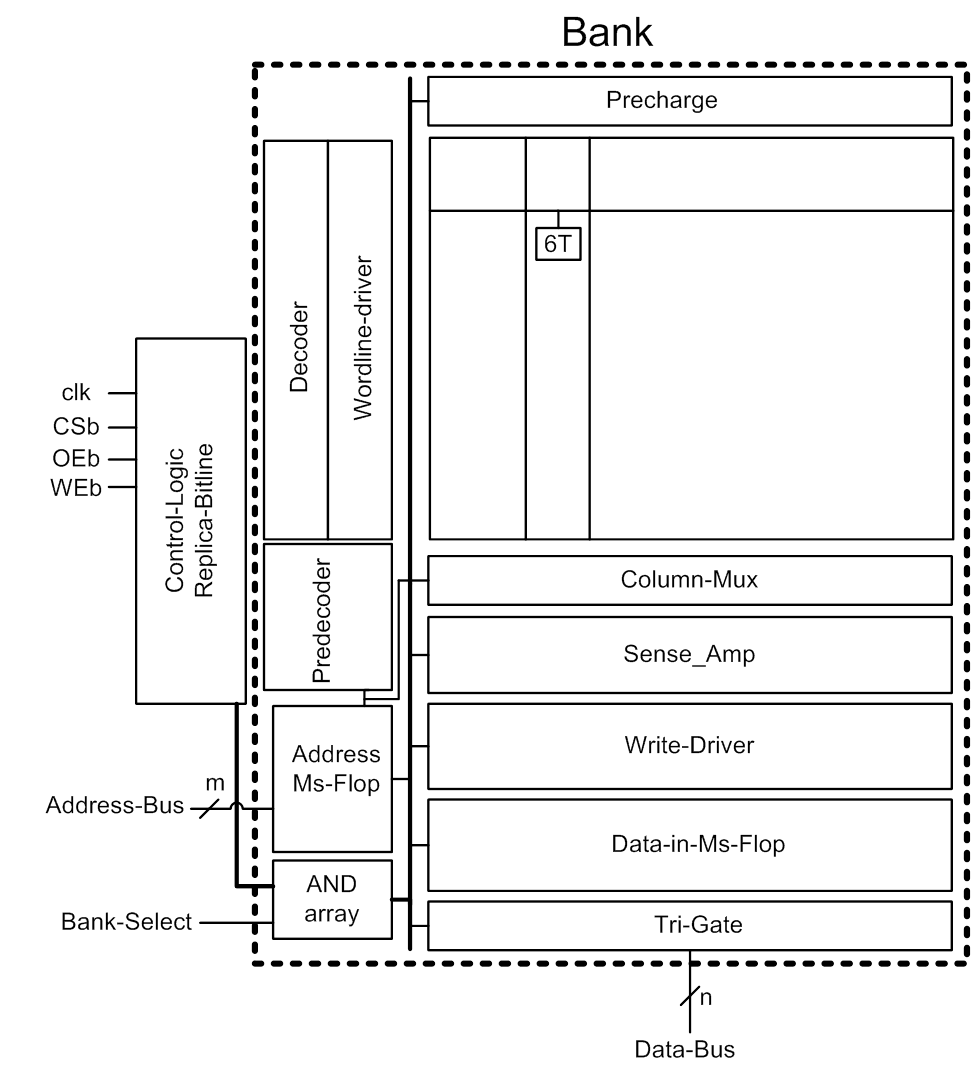
\includegraphics[scale=1]{./figs/bank.pdf}
\caption{Overal bank and SRAM architecture.}
\label{fig:bank}
\end{figure}


In order to reduce the delay and power, divided wordline strategy have been used in this compiler. Part of the address bits 
are used to define the global wordline (bank-select) and rest of address bits are connected to hierarchical 
decoder inside each bank to generate local wordlines that actually drive the bitcell access transistors. 

As shown in figure~\ref{fig:bank2} SRAM is divided to two banks which share data-bus, address-bus, control-bus and control-logic. 
In this case one bit of address (most significant bit) goes to an ms-flop and outputs of ms-flop (address-out and address-out-bar) 
are connected to banks as bank-select signals. Control logic is shared between two banks and based on which bank is selected, 
control signals will activate modules inside the selected bank. In this architecture, the total cell capacitance is reduced by up 
to a factor of two. Therefore the power will be reduced greatly and the delay among the wordlines is also reduced.

\begin{figure}[h!]
\centering
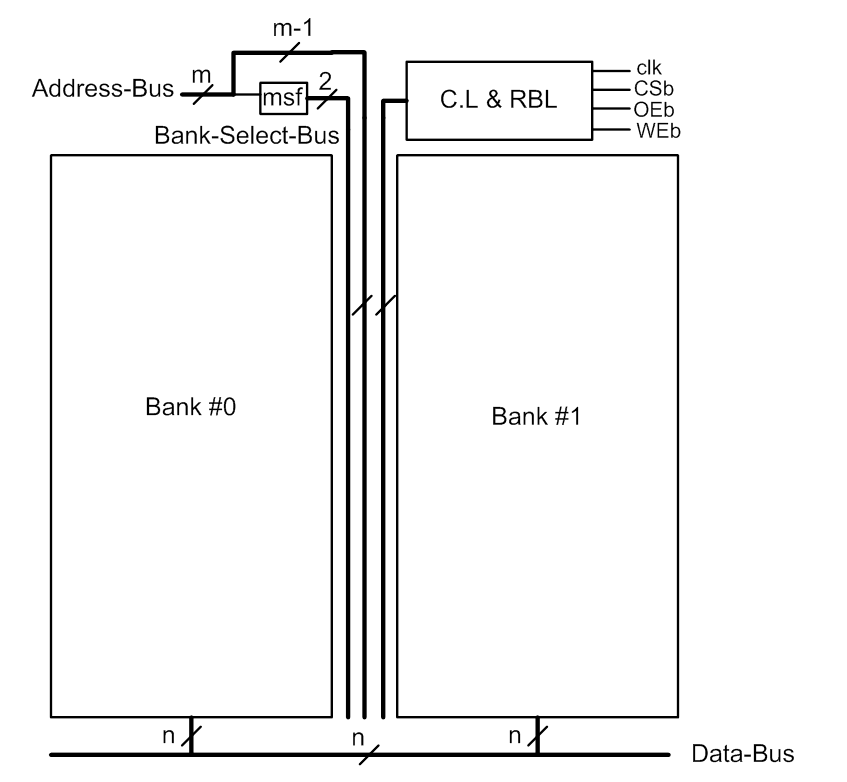
\includegraphics[scale=.9]{./figs/bank2.pdf}
\caption{SRAM is divided to two banks which share the control-logic.}
\label{fig:bank2}
\end{figure}

In figure~\ref{fig:bank4}, four banks are connected together. In this case a 2:4 decoder is added to select one of the banks using two 
most significant bits of input address. Control signals are connected to all banks but will turn on only the selected bank.


\begin{figure}[h!]
\centering
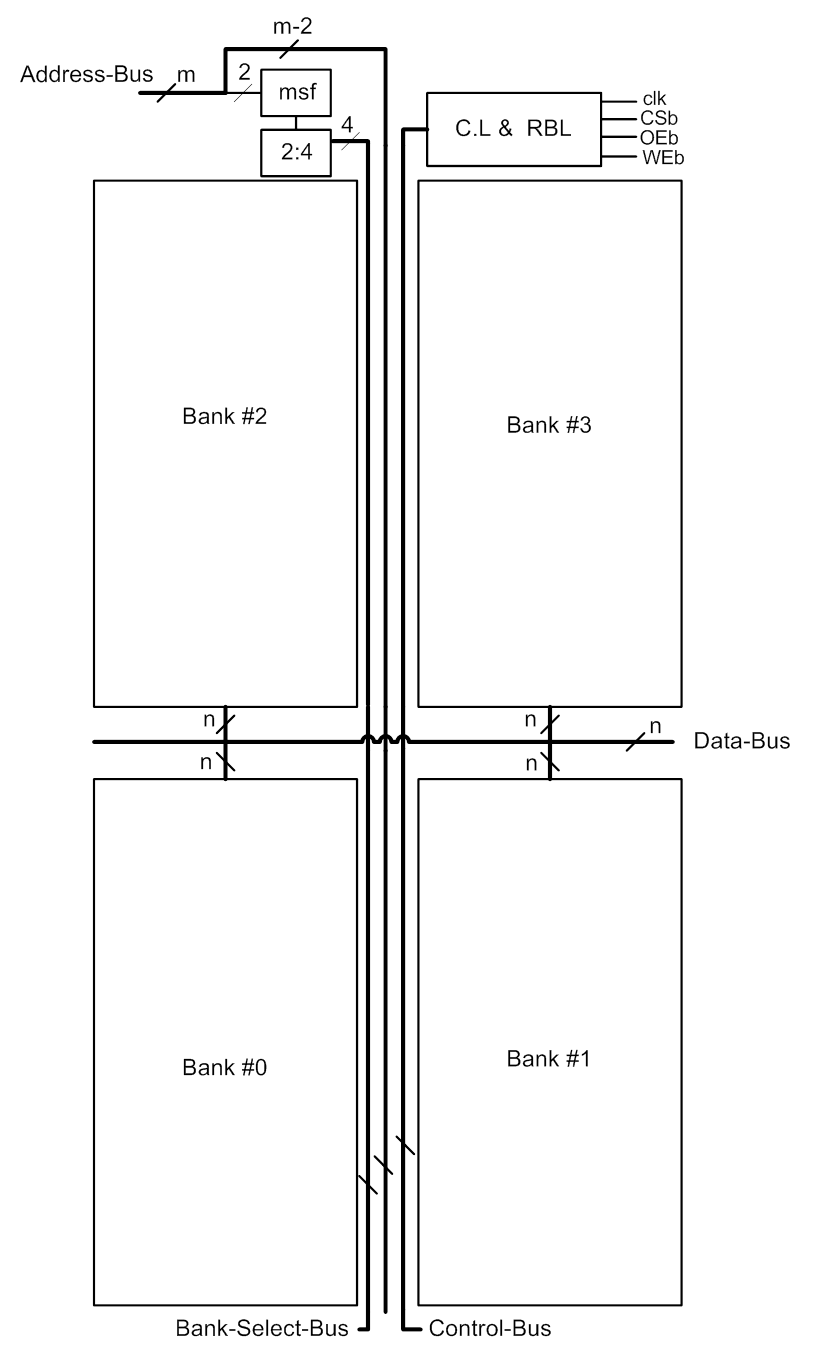
\includegraphics[scale=.9]{./figs/bank4.pdf}
\caption{SRAM is divided to 4 banks wich are controlled by the control-logic and a 2:4 decoder.}
\label{fig:bank4}
\end{figure}


